\documentclass[a5paper]{book} % draft,
\usepackage[top=1.5cm, bottom=1.5cm, left=2cm, right=2cm]{geometry} % showframe,
\usepackage{lmodern}
\usepackage{fancyhdr}
\usepackage[icelandic, czech, english]{babel}
\usepackage[utf8x, utf8]{inputenc}
\usepackage[T1]{fontenc}
\usepackage{hanging}
\usepackage{tikz}
\usetikzlibrary{calc}
\newcommand\entry[3][]{\hangpara{2em}{1}{\fontfamily{phv}\selectfont{\textbf{{#2}}}}\ 
#3\ifx\relax#1\relax\markboth{#2}{#2}\else\markboth{#1}{#1}\fi
\par}\nopagebreak[4]
\newcommand*{\dictchar}[1]{\centerline{\Huge\textbf{#1}}\par\vspace{1cm}}
% use fancyhdr or whatever you want to add
% the boxes to the header to make them appear
% on every page
\pagestyle{fancy}
% new counter to hold the current number of the
% letter to determine the vertical position
\newcounter{letternum}
% newcounter for the sum of all letters to get
% the right height of a box
\newcounter{letterdiv}
\setcounter{letterdiv}{26}
% some margin settings
\newlength{\thumbtopmargin}
\setlength{\thumbtopmargin}{1cm}
\newlength{\thumbbottommargin}
\setlength{\thumbbottommargin}{3cm}
% calculate the box height by dividing the page height
\newlength{\thumbheight}
\pgfmathsetlength{\thumbheight}{%
(\paperheight-\thumbtopmargin-\thumbbottommargin)%
/%
\value{letterdiv}
}
% box width
\newlength{\thumbwidth}
\setlength{\thumbwidth}{1.5cm}
% style the boxes
\tikzset{
thumb/.style={
   fill=black!50!red,
   text=white,
   minimum height=\thumbheight,
   text width=\thumbwidth,
   outer sep=0pt,
   font=\sffamily\bfseries,
}
}
\newcommand{\oddthumb}[1]{%
    % see pgfmanual.pdf for more information about this part
    \begin{tikzpicture}[remember picture, overlay]
        \node [thumb,text centered,anchor=north east,] at ($%
            (current page.north east)-%
            (0,\thumbtopmargin+\value{letternum}*\thumbheight)%
        $) {#1};
   \end{tikzpicture}
}
\newcommand{\eventhumb}[1]{%
    % see pgfmanual.pdf for more information about this part
    \begin{tikzpicture}[remember picture, overlay]
        \node [thumb,text centered,anchor=north west,] at ($%
            (current page.north west)-%
            (0,\thumbtopmargin+\value{letternum}*\thumbheight)%
        $) {#1};
   \end{tikzpicture}
}
% create a new command to set a new lettergroup
\newcommand{\lettergroup}[1]{%
\fancypagestyle{chapterstart}{%
\fancyhf{}
\renewcommand{\headrulewidth}{0pt}
\chead{\oddthumb{#1}}% chapters start only on odd pages
\cfoot{\thepage}
}
\fancyhead[LO]{\fontfamily{phv}\selectfont{\textbf{\rightmark}}\oddthumb{#1}}%
\fancyhead[RE]{\fontfamily{phv}\selectfont{\textbf{\leftmark}}\eventhumb{#1}}%
% step the counter of the letters
\stepcounter{letternum}%
}
\fancypagestyle{basicstyle}{%
\fancyhf{}
\renewcommand{\headrulewidth}{0.4pt}
\renewcommand{\footrulewidth}{0pt}
\fancyhead[LE,RO]{\textbf{\chaptitle}}
\fancyhead[LO,RE]{\textbf{\thepage}}}
\fancypagestyle{dictstyle}{%
\renewcommand{\headrulewidth}{0.4pt}
\fancyhf{}
\fancyhead[LE,LO]{{\fontfamily{phv}\selectfont{\textbf{\rightmark}}}}
\fancyhead[CO,CE]{\thepage}
\fancyhead[RE,RO]{{\fontfamily{phv}\selectfont{\textbf{\leftmark}}}}}
\setlength{\columnsep}{20pt}
\setlength{\columnseprule}{0.1pt}

\begin{document}
\pagestyle{dictstyle}
\fontfamily{lmss}\selectfont
\centering
\huge

\lettergroup{A}
\dictchar{A}
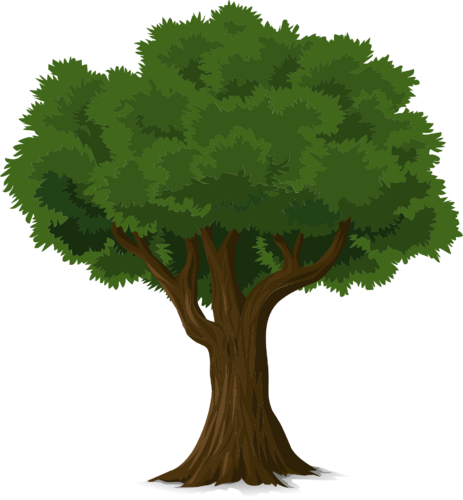
\includegraphics[width=\linewidth]{images/arbre}
L'arbre est vert

\clearpage
\lettergroup{B}
\dictchar{B}
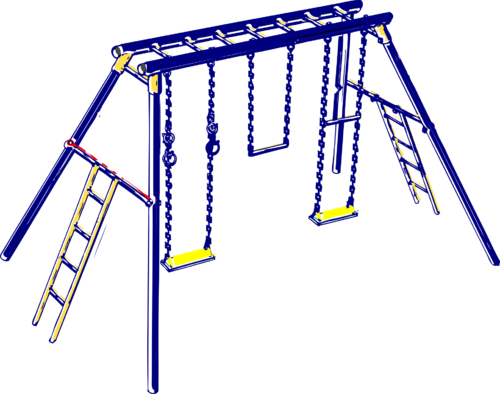
\includegraphics[width=\linewidth]{images/balancoire}
La balançoire est bleue

\clearpage
\lettergroup{C}
\dictchar{C}

\includegraphics[width=\linewidth]{images/coeur}
Le cœur est rouge

\clearpage
\lettergroup{D}
\dictchar{D}

\includegraphics[width=\linewidth]{images/droite}
La droite est bleue

\clearpage
\lettergroup{E}
\dictchar{E}

\clearpage
\lettergroup{F}
\dictchar{F}

\includegraphics[width=0.8\linewidth]{images/fraise}

La fraise est rouge

\clearpage
\lettergroup{G}
\dictchar{G}
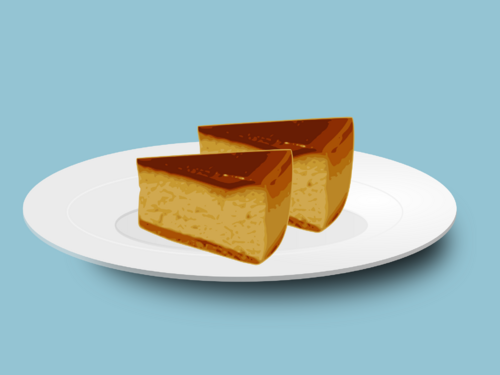
\includegraphics[width=\linewidth]{images/gateau}
Le gâteau est marron

\clearpage
\lettergroup{H}
\dictchar{H}

\clearpage
\lettergroup{I}
\dictchar{I}

\clearpage
\lettergroup{J}
\dictchar{J}

\clearpage
\lettergroup{K}
\dictchar{K}

\clearpage
\lettergroup{L}
\dictchar{L}

\clearpage
\lettergroup{M}
\dictchar{M}
Maman

\clearpage
\lettergroup{N}
\dictchar{N}

\includegraphics[width=\linewidth]{images/non}
Non

\clearpage
\lettergroup{O}
\dictchar{O}

\includegraphics[width=\linewidth]{images/oui}
Oui

\clearpage
\lettergroup{P}
\dictchar{P}
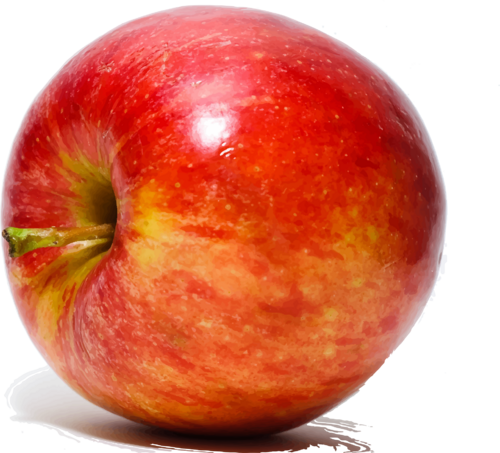
\includegraphics[width=\linewidth]{images/pomme}
La pomme est rouge

\clearpage
\lettergroup{Q}
\dictchar{Q}

\includegraphics[width=\linewidth]{images/quiche}
La quiche est jaune

\clearpage
\lettergroup{R}
\dictchar{R}

\includegraphics[width=\linewidth]{images/rose}
La rose est rouge

\clearpage
\lettergroup{S}
\dictchar{S}
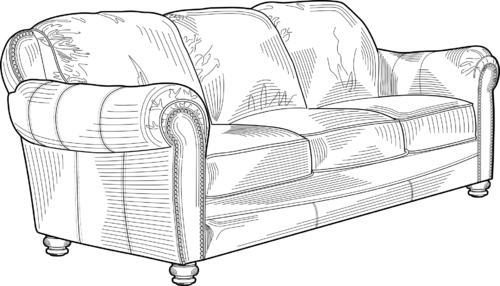
\includegraphics[width=\linewidth]{images/sofa}
Le sofa est noir

\clearpage
\lettergroup{T}
\dictchar{T}
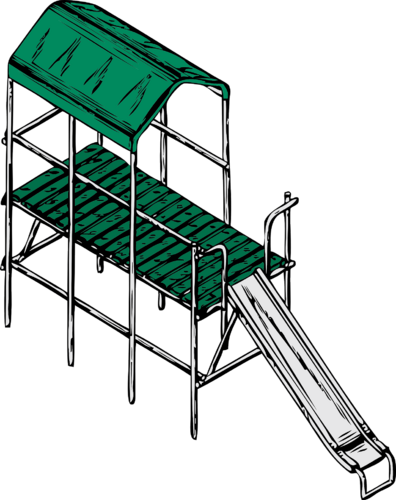
\includegraphics[width=\linewidth]{images/toboggan}
Le toboggan est blanc

\clearpage
\lettergroup{U}
\dictchar{U}

\clearpage
\lettergroup{V}
\dictchar{V}
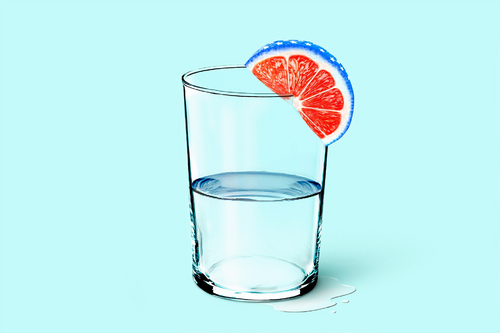
\includegraphics[width=\linewidth]{images/verre}
Le verre est transparent

\clearpage
\lettergroup{W}
\dictchar{W}

\clearpage
\lettergroup{X}
\dictchar{X}

\clearpage
\lettergroup{Y}
\dictchar{Y}

\clearpage
\lettergroup{Z}
\dictchar{Z}

\end{document}